%% Los cap'itulos inician con \chapter{T'itulo}, estos aparecen numerados y
%% se incluyen en el 'indice general.
%%
%% Recuerda que aqu'i ya puedes escribir acentos como: 'a, 'e, 'i, etc.
%% La letra n con tilde es: 'n.

\chapter{Radar de Apertura Sintética}
\label{Radar}

Los sistemas de Radar (radio detection and ranging: detección y medición de distancias por radio) son instrumentos que, a través de ondas electromagnéticas, detectan un objeto e indican su distancia y posición. 
Estos instrumentos miden la respuesta del blanco a la radiación electromagnética emitida en forma de pulsos, el valor de esta respuesta es almacenada para su posterior procesamiento y se utiliza para formar una imagen de la zona de interés. A diferencia de los sensores ópticos e infrarrojos que son inherentemente pasivos, el radar es un sensor activo, proporciona su propia iluminación en forma de microondas. Las microondas son ondas electromagnéticas (EM) que se encuentran en aproximadamente la zona de $1$ a $300$ GHz del EM, es decir, longitudes de onda entre $1$ centímetros a $1$ milímetro.

Muchos de los radares montados sobre plataformas móviles son de vista lateral (SLAR: Side Looking Airbone Radar), dentro de éstos podemos encontrar los radares de apertura real (RAR: Real Aperture Radar) y los radares de
apertura sintética (SAR: Synthetic Aperture Radar). 

¿Por qué vista lateral? Porque los retornos porvenientes de distintos puntos del terreno llegarán en tiempos diferentes, ya que difieren en su distancia al radar. En cambio, en los radares de vista vertical, se pueden recibir señales provenientes de puntos equidistantes. Esto llevaría a ambigüedades ya que el tiempo de arribo de la señal sería el mismo para este tipo de sensores.

¿Por qué SAR y no RAR? La resolución en la dirección del desplazamiento $(\Delta x)$ es la mínima distancia que tienen que tener dos puntos diferentes en el terreno para que el sensor sea capaz de distinguirlos. Los sensores RAR tienen un baja resolución espacial, ésta se define como  $\Delta x\approx\dfrac{\lambda \cdot r}{L}$ ~\cite{Sarmap2009}, donde $\lambda$ es la longitud de onda  de la señal emitida, $r$ la altura entre el sensor y el terreno y $L$ la longitud de la antena. Esto se muestra en la figura~\ref{Resolucion}.

\begin{figure}[hbt]
	\centering    
	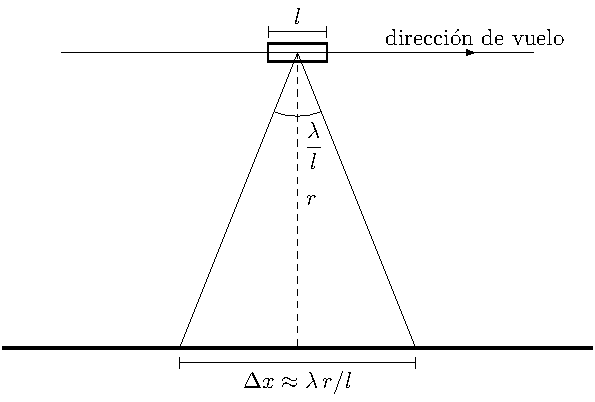
\includegraphics[scale=1]{../../Figures/Tesis/Capitulo3/Resolucion.pdf}
	\caption{\label{Resolucion}Resolución de un radar.}
\end{figure} 

De esta manera para disminuir el valor de $\Delta x$, es decir, aumentar la resolución es necesario disminuir $r$, $\lambda$ o aumentar $L$. Los sensores ópticos son los que emiten radiación electromagnética con una longitud de onda menor a la correspondiente a microondas. La ventaja de esto es aumentar la resolución a expensas de las condiciones climáticas entre otros factores.

La tecnología SAR permite simular una antena más larga aprovechando que estos sensores son aerotransportados. Cuando un blanco se mueve con respecto a la fuente de emisión de ondas se observa un desplazamiento en frecuencia entre la señal emitida y la recibida. Esta diferencia en frecuencia se conoce como efecto Doppler y afecta la frecuencia observada cuando hay un movimiento relativo entre el objeto y el sensor. La teconología SAR hace uso del efecto Doppler para generar una apertura virtual más grande que la real, por eso se llama de apertura sintética.

Este tipo de imágenes son de gran utilidad ya que permiten obtener información sobre recursos naturales, como así también, permiten detectar efectos de la acción del hombre tales como deforestación, cultivos y embalses. Además presentan ventajas y desventajas sobre las imágenes obtenidas por sensores ópticos, entre las que se encuentran 

\medskip

Ventajas:
\begin{itemize}
	\item El radar posee un sistema de iluminación propio que permite la adquisición de imágenes tanto de día como de noche.
	\item Los sistemas SAR emiten radiación electromagnética a frecuencias que permiten atravesar las nubes sin pérdida en la calidad de la imagen obtenida, como así también atravesar zonas de forestación obteniendo mayor información de la zona bajo estudio.
\end{itemize}

Desventajas: 
\begin{itemize}
	\item Las imágenes SAR tienen la desventaja de poseer un ruido que es inherente al proceso de captura de la imagen, ya que el tipo de iliminación que se utiliza para formar la misma es de tipo coherente \cite{goodman85}. Este ruido, llamado speckle, es multiplicativo, no gaussiano y, por lo tanto, diferente al ruido que se observa en imágenes ópticas. La presencia de este ruido hace que en este tipo de imágenes se observen, en algunos casos, un granulado o falta de contraste.
\end{itemize}
%Entonces debido a la gran velocidad de desplazamiento de la plataforma que transporta al sensor, la antena del dispositivo SAR se convierte en una antena virtual mucho más grande que la que tiene en realidad, por eso se llaman de apertura sintética.

En este capítulo presentamos una breve descripción del funcionamiento de un radar de apertura sintética y de la forma en que se adquieren este tipo de imágenes, ya que éstas son el objeto de estudio en esta tesis.



%%%%%%%%%%%%%%%%%%%%%%%%%%%%%%%%%%%%%%%%%%%%%%%%%%%%%
%Azimut es la dirección paralela a la trayectoria de vuelo de la aeronave. La Figura 3 muestra que la extensión angular del haz de radar en la dirección de acimut es igual a H / La, donde es la longitud de onda del haz transmitido y La es la longitud de la antena de radar en la dirección de azimut. Esta propagación es debido a la interferencia de las ondas emitidas desde y recibidas por los dipolos de la antena, lo que provoca la propagación angular a disminuir a medida que aumenta la longitud de apertura (de antenas largas produce un haz apretado, tanto como un largo cañón de un arma produce menos dispersión). Dos objetos en el suelo y con la misma inclinación gama R solamente se pueden obtener imágenes por separado si no lo son tanto dentro del haz del radar al mismo tiempo. Así, la resolución de acimut es
%
%
%Un Radar de Apertura Sintética (synthetic aperture radar: SAR) es un tipo de sistema que consiste en procesar, mediante algoritmos, la información capturada por la antena del radar. Debido a la gran velocidad de desplazamiento del vehículo que transporta el radar, la antena del dispositivo SAR  se convierte en una antena virtual mucho más grande que la que tiene en realidad, por eso se llaman de apertura sintética. 
%% % % ACF ¿Qué "rendimiento"? ¿Sería resolución espacial?
%
%%Formulado ya en 1891 por la American Hugo Gernsback, el radar
%%principio ( "Radio Detection and Ranging") se basa en los principios de
%%La propagación electromagnética: una onda electromagnética emitida por una fuente es
%%retrodispersada por objetivos. La señal recibida, una vez analizada, hace que sea posible
%%detectar y localizar estos objetivos, suponiendo que la velocidad de propagación de la
%%Wave se mantiene bastante constante.
%
%Los radares RAR tienen una baja resolución espacialla resolución azimutal es directamente proporcional a la distancia entre la antena y el albo imageado, e inversamente proporcional a la longitud de onda de la antena utilizada para el imageamiento. De esta forma, para obtener una mejor resolución azimutal es preciso disminuir la distancia entre el radar y el albo o aumentar la longitud de la antena.
%
%VER
%%El mayor problema de los sensores RAR radica en su baja resoluci´on espacial
%%como consecuencia del escaso di´ametro de la antena, donde el tama˜no
%%m´ınimo del objeto identificable en la imagen est´a en relaci´on directa con la
%%longitud de onda y la altura de observaci´on y es inversamente proporcional
%%al di´ametro de la apertura. En una plataforma espacial, ser´ıa imposible lograr
%%una buena resoluci´on con este sistema, dado que ser´ıa preciso contar con
%%antenas de enormes proporciones.
%%La señal recibida por el radar es un número complejo, a partir de esta señal se forma la imagen. Si consideramos el módulo de la señal recibida decimos que los datos están dados en formato amplitud, en cambio, si utilizamos el cuadrado del módulo de dicha señal diremos los datos están dados en formato intensidad. En esta tesis se trabajará con los datos dados en este último formato.



%%%%%%%%%%%%%%%%%%%%%%%%%%%%%%%%%%%%%%%%%%%%%%%%%%%%%%%%%%%%%%%%%%%%%%%%%%%%%%%%%%%%
%Explicar qué es un sistema de iluminación coherente

%poner imágenes con ruido speckle y sin ruido
%%%%%%%%%%%%%%%%%%%%%%%%%%%%%%%%%%%%%%%%%%%%%%%%%%%%%%%%%%%%%%%%%%%%%%%%%%%%%%%%%%%%

\section{Sensores Remotos SAR}

\textcolor{red}{Acá poner algo de historia de los sensores, e ir directamente a los más importantes actualmente. Hay que dar detalles de aquellos de los cuales usamos imágenes.}

Un radar de apertura sintética SAR es un sensor activo que ilumina la escena emitiendo señales en la región de microondas del espectro electromagnético.

Antes del desarrollo de las imágenes de radar, las imágenes de alta resolución provenían de sensores pasivos que son sensibles tanto a la radiación solar como a la térmica emitida por la superficie de la tierra. Por lo tanto estos sensores necesitan de una fuente de iluminación externa para poder captar el objetivo de interés. 

Los sensores SAR poseen una tecnología diferente para obtener información de la superficie terrestre. Estos sensores son activos, es decir, poseen un sistema de iluminación propia que les permite obtener imágenes en forma independiente de la luz solar. Esto aumenta la capacidad de obtener imágenes ya que pueden operar en forma continua durante el día y la noche.

Dado que estos sistemas emiten puslos en el espectro de las microondas, ni las nubes, ni la niebla, ni las precipitaciones impiden la adquisición de imágenes. Esto hace que los sensores SAR puedan operar en forma independiente de las condiciones climáticas. Por lo tanto estos instrumentos son capaces de obtener información de la tierra en forma continua lo que permite observar fenómenos como corrientes oceánicas, detectar cambios en la vegetación o moviemientos del hielo.

%Como se indica en~\cite{Maitre2010} los primeros experimentos de detección de aeronaves datan de 1934. Esto explica por qué tanto los británicos como estadounidenses y alemanes  tales sistemas durante la 2ª Guerra Mundial. 

De acuerdo a~\cite{Moreira2013}, durante los años $50$ y $60$ la investigación militar utilizó ampliamente los sistemas SAR con el propósito del reconocimiento del terreno. Sin embargo, a partir de los años $70$ y $80$ se desarrollaron varios sensores SAR aerotransportados  para aplicaciones civiles con el objetivo final de recuperar parámetros geo/biofísicos y detectar cambios en la superficie terrestre.

El primer satélite civil que tuvo a bordo un radar SAR fue lanzado en $1978$~\cite{Seasat} a fines de junio por el Jet Propulsion Laboratory (JPL) de la NASA. Este satélite fue diseñado para teledetección de los océanos de la tierra, registrando información de los vientos de la superficie marina y la temperatura, altura de las olas, características hielo marino entre otros parámetros de interés. Debido a un problema eléctrico, este satélite finalizó sus operaciones a mediados de octubre del mismo año.


La Comisión Nacional de Actividades Espaciales (CONAE) y el INVAP de Argentina, junto con la Agencia Espacial Italiana (ASI) integran el Sistema Ítalo Argentino de Satélites para la Gestión de Emergencias (SIASGE)~\cite{Invap}. De acuerdo a~\cite{Saocom} el objetivo de la misión SAOCOM es la puesta en órbita de dos constelaciones: SAOCOM1 y SAOCOM2. Cada constelación se compone de dos satélites llamados A y B. El satélite SAOCOM1A fue puesto en órbita el 7 de octubre de 2018 en Vanderberg, California. En~\cite{Saocom} se puede ver un video de su lanzamiento.

Entre los objetivos de estos satélites se encuentra la medición de la humedad del suelo, detectar derrames de hidrocarburos en el mar y el seguimiento de la cobertura de agua en las inundaciones. Están equipados con tecnología SAR polarimétrica y operan en banda L. La banda L permite penetrar a través de la superficie hasta $2$ m de profundidad dependiendo del tipo de suelo. 

En la tabla~\ref{tabla:SensoresSAR}, y de acuerdo a la información obtenida de~\cite{Moreira2013}, se muestran los principales sensores SAR junto con el período, banda y frecuencia de operación y las instituciones/países que lo desarrollaron. 

\begin{table}[H]
	\centering
	\begin{spacing}{1.25}
		\begin{tabular}{l*4{l}}
			\toprule
			\multirow{2 }{*} {Sensor}       &	\multirow{2 }{*} {Operación	}   	&	Banda y 	            		 &	\multirow{2 }{*} {Institución/País} \\
			&                       				&   Polarización            		 &                     \\
			\midrule
			Seasat	                        &	1978	            				&	L (HH)	                		 &	NASA/JPL, USA \\
			ERS -1/2	                    &	1991–2000/1995–2011					&	C (VV)	                		 &	ESA, Europe \\
			J-ERS -1	                    &	1992–1998	        				&	L (HH)	                		 &	JAXA, Japan \\
			Radarsat-1   	                &	1995-2013   	    				&	C (HH)	                 		 &	CSA, Canada \\
			\multirow{2 }{*} {SRTM}	        &	\multirow{2 }{*} {Lanzado en 2000}  &	C (HH+VV) 				         &	NASA/JPL, USA, DLR,  \\
			&                       				&   y X (VV)                   		 &   Germany, ASI, Italy\\
			ENVISAT / ASAR	                &	2002–2012   	    				&	C (dual)	                		 &	ESA, Europe \\
			ALOS /PalSAR	                &	2006–2011   	   					&	L (quad)	             		 &	JAXA, Japan \\
			TerraSAR -X/	                &	Lanzado en 2007	  				    &	\multirow{2 }{*} {X (quad)}	     &	\multirow{2 }{*} {SDLR/Astrium,Germany} \\
			TanDEM -X	                    &	Lanzado en 2010   				 	&	            			         &	             \\
			Radarsat-2	                    &	Lanzado en 2007    					&	C (quad)            		     &  CSA, Canada	 \\
			COSMO -SkyMed-1/4	            &	Lanzado en 2007	    				&	X (dual)          			     &	ASI/MiD, Italy \\
			RISAT -1	                    &	Lanzado en 2012   				 	&	C (quad)            			 &	ISRO, India \\
			\multirow{2 }{*} {HJ-1C	}       &	\multirow{2 }{*} {Lanzado en 2012} 	&	\multirow{2 }{*} {S (VV)}		 &	CRESDA/CAST / \\
			&                       				&                             		 &  NRSCC, China                   \\
			Kompsat-5	                    &	Lanzado en 2013	  				    &	X (dual)            			 &	KARI, Korea \\
			PAZ	                            &	Lanzado en 2018   				 	&	X (quad)            		     &	CDTI, Spain \\
			ALOS -2	                        &	Lanzado en 2014	 				    &	L (quad)            		     &	JAXA, Japan \\
			Sentinel-1a/1b              	&	Lanzado en 2014    				    &	C (dual)            			 &	ESA , Europe \\
			Radarsat 	                    &	\multirow{2 }{*} {Lanzado en 2019}  &	\multirow{2 }{*} {C (quad) }     &	\multirow{2 }{*} {CSA, Canada }\\
			Constellation-1/2/3             &                   			        &   			          			 &                     \\
			SAOCOM -1/2	                    &	Lanzado en 2018  					&	L (quad)	           			 &	CONAE, Argentina \\
			\bottomrule
		\end{tabular}
	\end{spacing}
	\caption{\label{tabla:SensoresSAR}Descripción de algunos sensores SAR junto con sus características. Adaptado de Moreira et al.~\cite{Moreira2013}.}
\end{table}

\section{Sistema de iluminación coherente}
\label{coherente}


Un haz de luz esta formado por ondas electromagnéticas cuya longitud de onda está comeprendida entre $400$ y $800$ nanómetros.

La superposición de dos o más ondas producen diferentes tipo de sistemas de iluminación, esto se muestra la figura~\ref{LuzCoherente}.

\begin{figure}[hbt]
	\centering    
	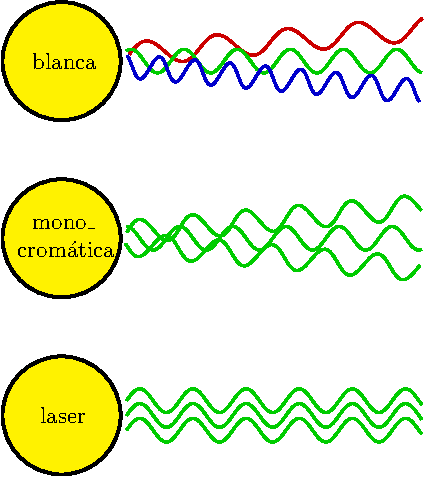
\includegraphics[scale=0.7]{../../Figures/Tesis/Capitulo3/LuzCoherenteTico.pdf}
	\caption{\label{LuzCoherente}Diferentes tipos de sistemas de iluminación.}
\end{figure} 

Cuando se suman dos o más señales se superponen de manera constructiva o destructiva, produciendo de esta forma intensidades máximas o mínimas. Una luz con estas características se denomina incoherente como lo es la luz blanca.

En cambio, con una fuente de luz coherente en frecuencia, todas las ondas emitidas tienen la misma longitud de onda. A este tipo de señal se llama luz monocromática. Si además estas señales tienen una diferencia de fase constante en el tiempo serán coherentes en fase. 

Las señales emitidas por un laser o por un radar de apertura sintética son coherentes en fase, en frecuencia, y además los máximos de la señal se producen al mismo tiempo. Esto se conoce como sistema de iluminación coherente.

\section{Espectro Electromagnético}

Las ondas electromagnéticas se modelan con una sinusoidal donde la longitud de onda $\lambda$ es la distancia entre los máximos de la sinusoide. La frecuencia $f$ de la onda es el número de máximos por unidad de tiempo. Estas medidas están relacionadas por la ecuación $c=\lambda \cdot f$ donde $c$ es la velocidad de la luz. De esta ecuación vemos que $\lambda$ y $f$ están inversamente relacionadas dado que $c$ es un valor constante.
%, estos parámetros se muestran en la figura~\ref{LongOnda}
%\begin{figure}[H]
%	\centering    
%	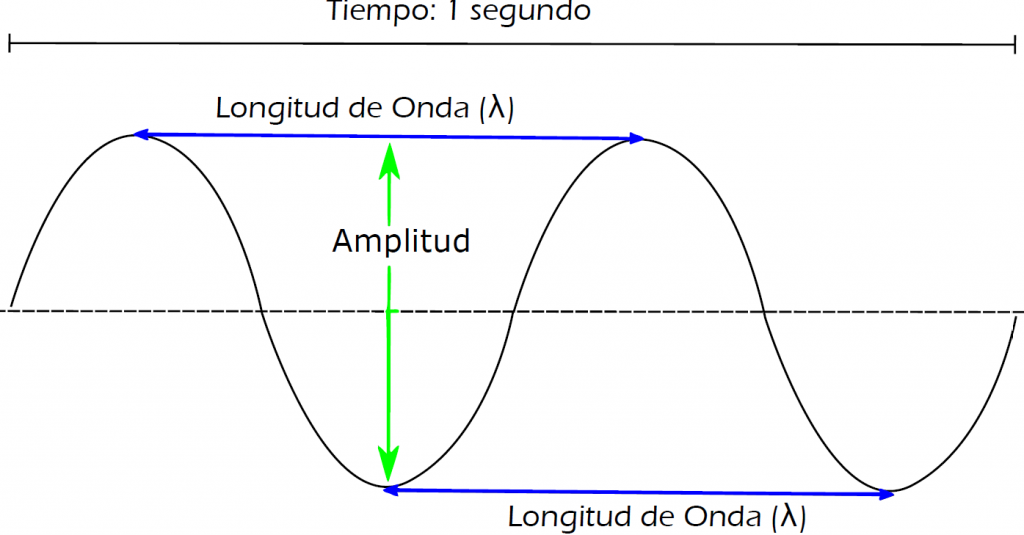
\includegraphics[scale=0.5]{../../Figures/Tesis/Capitulo3/LongOnda.png}
%	\caption{\label{LongOnda}Parámetros de una señal.}
%\end{figure} 

Como dijimos anteriormente el radar SAR emite señales en la región de microondas del espectro electromagnético (EM) y en diferentes bandas. La figura~\ref{Espectro} muestra cómo está formado el EM de acuerdo a la longitud de onda de la señal.

\begin{figure}[hbt]
	\centering    
	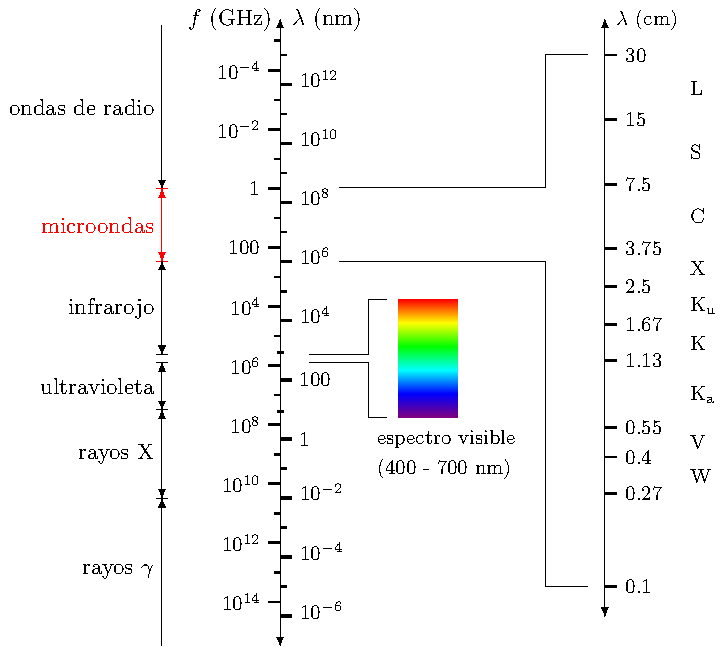
\includegraphics[scale=1]{../../Figures/Tesis/Capitulo3/EEM.pdf}
	\caption{\label{Espectro}Espectro electromagnético.}
\end{figure}

Las microondas, que son parte del espectro electromagnético, tienen longitudes de onda considerablemente más grande que la luz visible. Un aspecto a tener en cuenta al momento de elegir una longitud de onda es la penetración. Cuanto más grande es la longitud de onda (frecuencias más chicas), más fuerte es la penetración en la vegetación y el suelo. La tabla~\ref{Bandas} se presentan las bandas más usadas en teledetección por microondas.

\begin{table}[H]
	\centering
	\begin{tabular}{ccc}
		\toprule
		\textbf{Banda}	& \textbf{Frecuencia}		    	& \textbf{Longitud de onda} \\ \midrule
		X-band			& 12.5 a 8 \si{\giga\hertz}         &  2.4 a 3.75 \si{\centi\meter} \\
		C-band			&  8 a 4 \si{\giga\hertz} 			&  3.75 a 7.5 \si{\centi\meter}\\
		S-band			&  4 a 2 \si{\giga\hertz} 	        &  7.5 a 15 \si{\centi\meter} \\
		L-band			&  2 a 1 \si{\giga\hertz} 	        &  15 a 30 \si{\centi\meter} \\
		P-band			&  0.999 a 0.2998 \si{\giga\hertz} 	&  30 a 100 \si{\centi\meter} \\
		\bottomrule
	\end{tabular}
	\caption{\label{Bandas}Bandas SAR, datos adaptados de~\cite{Sarmap2009}}
\end{table}

Cada banda es utilizada en diferente tipos de aplicaciones:

\begin{description}
\item[X-band:] se utiliza para tener imágenes de alta resolución.
\item[C-band:] atraviesa las nubes y la lluvia.
\item[S-band:] útil para medir niveles de precipitación.
\item[L-band:] útil para aplicaciones en agricultura y mediciones de humedad del suelo.
\item[P-band:] adecuada para  imágenes con importante penetración en la vegetación.
\end{description}

%La energía en el espectro de las microondas es útil en teledetección porque es capaz de atravesar la atmósfera bajo prácticamente todas las condiciones climáticas (niebla, lluvia, nieve, nubes). 

\section{Polarización}

Las ondas electromagnéticas son ondas transversales, es decir, la dirección del vector campo eléctrico $\vec{\mathbf{E}}$ es perpendicular a la dirección de propagación de la onda. Un aspecto a tener en cuenta es la polarización de una onda electromagnética, que se define como la orientación del vector campo eléctrico $\vec{\mathbf{E}}$ de la radiación transmitida o recibida. La luz correspondiente al espectro visible por lo general no está polarizada, todas las direcciones de $\vec{\mathbf{E}}$ son igualmente probables en el plano perpendicular a la dirección de propagación de la onda. Si la señal se descompone en dos ondas de igual amplitud pero con una diferencia de fase de $90º$, entonces se dice que la luz está polarizada circularmente porque $\vec{\mathbf{E}}$ gira describiendo un círculo en el plano ortogonal a la dirección de propagación, a medida que la señal avanza. Si las dos ondas tienen diferente amplitud y están desfasadas entre sí $90º$, o si el desfasaje es distinto de $90º$, la luz se dice que está polarizada elípticamente. Cuando el vector $\vec{\mathbf{E}}$ se mantiene paralelo a una dirección fija la polarización se llama lineal. La figura~\ref{PolarizacionCircularLineal} muestra luz  circular o linealmente polarizada.
 %se puede ver en la figura~\ref{PolarizacionCircularEliptica} 

\begin{figure}[hbt]
	\centering    
	\subfigure[Polarización Circular\label{PolarizacionCircular}]{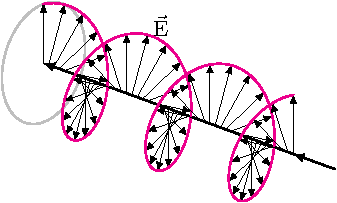
\includegraphics[scale=1]{../../Figures/Tesis/Capitulo3/PolarizacionCircular.pdf}} \qquad
	\subfigure[Polarización Lineal\label{PolarizacionCircular}]{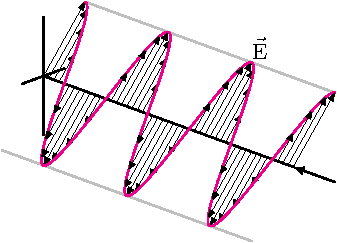
\includegraphics[scale=1]{../../Figures/Tesis/Capitulo3/PolarizacionLineal.pdf}}
	\caption{\label{PolarizacionCircularLineal}Diferentes tipos de polarizaciones.}
\end{figure} 

Los radares de teledetección generalmente están diseñados para transmitir radiación vertical u horizontalmente polarizada. 
%\begin{figure}[hbt]
%	\centering    
%	\includegraphics[scale=0.7]{../../Figures/Tesis/Capitulo3/Polarizacion.pdf}
%	\includegraphics[scale=0.7]{../../Figures/Tesis/Capitulo3/Polarizacion2.png}
%	\caption{\label{PolarizacionLineal}Polarización de las ondas electromagnéticas.}
%\end{figure} 

La antena del radar puede recibir radiación polarizada vertical u horizontalmente y, a veces, ambas. Los planos de polarización transmitida y recibida se designan con las letras H para horizontal y V para vertical. Por lo tanto, la polarización de una imagen de radar puede ser HH, para transmisión horizontal, recepción horizontal, VV para transmisión vertical, recepción vertical, HV para transmisión horizontal, recepción vertical y viceversa (VH).

En el caso donde la polarización de la radiación recibida coincide con la polarizacion de la radiación transmitida, se conoce como imagen polarizada de manera similar. En cambio, cuando la polarización de la radiación recibida es ortogonal a la polarización de la radiación transmitida, se dice que la polarización es cruzada.  

Los sistemas SAR monopolarizados operan con una única polarización de emisión y detecta una sola de las componentes de la radiación recibida. Generalmente usan polarización similar, es decir igual polarización al emitir y recibir,  porque las señales de polarización cruzada son demasiado débiles para producir una buena imagen. De esta forma podemos tener radares monopolares o monopolarimétricos HH, VV, HV o VH donde la primera letra indica la polarización de la radiación emitida y la segunda indica la componente de la radiación detectada. Los primeros sensores SAR, como por ejemplo,  RADARSAT-1, que ha sido sustituido por RADARSAT-2, adquieren imágenes únicamente en la banda C y en la combinación HH. 

Si un radar tiene la capacidad de captar distintas polarizaciones se lo identificará como polarimétrico. En este tipo de radares se emite una señal electromagnética con polarización horizontal y vertical y se detectan ambas polarizaciones en la radiación recibida. Es decir, operan en las cuatro combinaciones citadas al mismo tiempo generando, en principio, imágenes de cuatro bandas. En esta tesis trabajaremos con imágenes monopolarimétricas.

\section{Geometría SAR}

El radar de apertura sintética SAR  es un sensor activo, de vista lateral, que emite energía en un período corto de tiempo y en el  intervalo  de  frecuencias  de  microondas recibiendo la señal reflejada por el blanco iluminado. Está montado sobre una plataforma móvil (aeronave o satélite) que transmite y recibe las señales con la misma antena, la cual tiene su eje longitudinal paralelo a la trayectoria de vuelo. Debido a la gran velocidad del desplazamiento de la plataforma y aprovechando el efecto Doppler que tiene lugar como consecuencia de dicho desplazamiento, la antena del dispositivo SAR  se convierte en una antena virtual de mayor tamaño. 

El radar se desplaza a una velocidad $\vec{v}$ y a una altura $h$ portando una antena que emite radiación electromagnética e ilumina la superficie del terreno. En la figura~\ref{GeometriaSAR} se muestra un esquema del movimiento del radar, la región sombreada es la zona iluminada por el radar. Esta zona permanece en el haz de la antena durante unos instantes y es observado por el radar desde numerosos puntos a lo largo de la trayectoria de la plataforma.
%, lo que es equivalente a prolongar la longitud real de la antena.

Vamos a dar algunas definiciones sobre la geometría SAR:
\begin{itemize}
	\item Azimut: es la dirección paralela a la trayectoria de vuelo de la plataforma.
	\item Rango: es la dirección perpendicular a la trayectoria de vuelo de la aeronave, es decir, perpendicular al azimut.
	\item Nadir: es el punto de la superficie terrestre justo debajo del rada.
	\item Swath: es el ancho de la zona iluminada.
	\item Slant Range: es la distancia oblicua entre el objetivo y la antena del radar.
	%\item Ground Range: es la proyección sobre la tierra de la distancia entre el objetivo y la antena del radar.
\end{itemize}

\begin{figure}[hbt]
	%\label{Dispersion}
	\centering    
	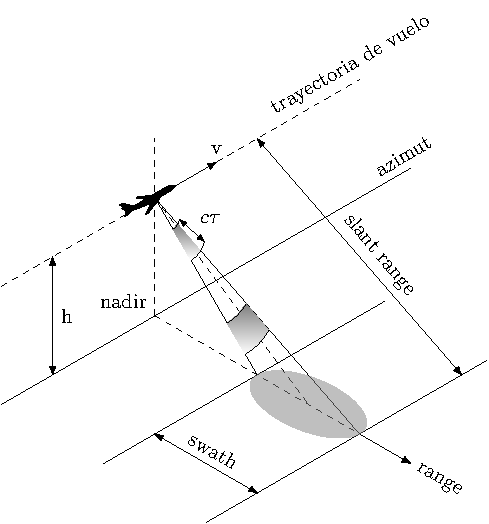
\includegraphics[scale=1]{../../Figures/Tesis/Capitulo3/sar_3d.pdf}
	\caption{\label{GeometriaSAR}Geometría del Radar de Apertura Sintética SAR.} %Fuente Canada Centre for Remote Sensing~\cite{ccrs2001}.}
\end{figure} 

La antena del radar tiene su eje longitudinal paralelo a la trayectoria de vuelo y emite pulsos de energía electromagnética perpendicular a dicha trayectoria, como se ilustra en la figura~\ref{GeometriaSAR}. Los pulsos electromagnéticos iluminan un área en el terreno, la antena recibe la energía reflejada en diferentes momentos, dependiendo de la distancia que existe entre el objeto y la antena. Con  al procesamiento de la señal reflejada se genera la imagen. 
A medida que el radar se desplaza emite pulsos de radiación electromagnética y recibe la señal correspondiente a la energía reflejada (retrodispersada)  por la superficie sensada. En el momento en el que este pulso incide sobre el blanco la radiación emitida sufre un proceso de dispersión como se muestra en la figura~\ref{SeñalDispersada} dependiendo del tipo de textura que tiene el blanco iluminado. 

\begin{figure}[H]
	%\label{Dispersion}
	\centering    
	\subfigure[Superficie Plana]{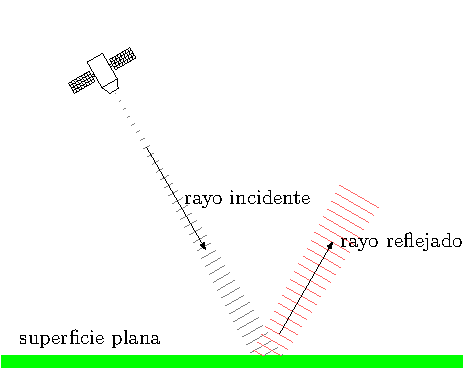
\includegraphics[scale=0.7]{../../Figures/Tesis/Capitulo3/superficie_plana_2.pdf}}
	\subfigure[Superficie Rugosa]{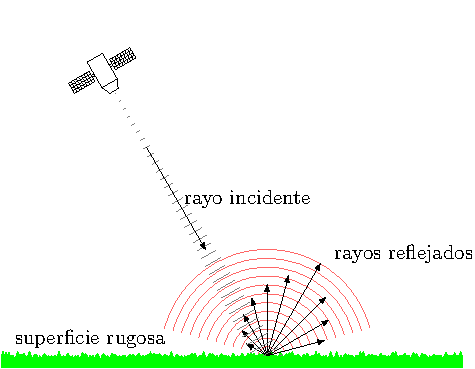
\includegraphics[scale=0.7]{../../Figures/Tesis/Capitulo3/superficie_rugosa.pdf}}
	\caption{\label{SeñalDispersada}Dispersión de la señal emitida por un radar SAR.}
\end{figure} 
%
\subsection{Resolución}

La resolución de un radar es la capacidad que tiene para distinguir la posición entre objetos que están muy cercanos en rango o en azimut. Entonces, la resolución se divide en dos categorías: resolución en rango y resolución en azimut. 

El grado de resolución en rango depende de la longitud temporal del pulso transmitido. Si el radar emite pulsos de longitud temporal $\tau$ la resolución en slant range queda determinada por $\Delta sl= \dfrac{c \tau}{2}$ donde $c$ es la velocidad de la luz~\cite{Sarmap2009,Moreira2013}. Entonces, señales con pulsos de longitud temporal pequeña mejoran la resolución en rango.
%, mientras que en ground range queda determinada por $\Delta gr= \dfrac{c \tau}{2 \sin \theta}$,

En los radares de apertura real RAR la resolución en azimut se define como $\Delta x_{\tiny \text{rar}}= R \ \dfrac{\lambda}{L}$ donde $R$ es la distancia del objeto al radar, $L$ es la longitud de la antena y $\lambda$ es el ancho de banda del pulso emitido por el sensor. Esto tiene el inconveniente de que la resolución depende de la distancia al sensor. Cuanto mayor es esta distancia mayor es el valor de $\Delta x_{\tiny \text{rar}}$ y, por lo tanto, menor la resolución. Con el fin de mejorar dicha resolución se debería disminuir el ancho de banda $\lambda$ o aumentar la longitud de la antena $L$. Si se reduce $\lambda$ dejamos de estar en el espectro de las microondas. Por otro lado la antena no puede ser excesivamente grande por razones de ingeniería estructural.

De acuerdo a~\cite{Moreira2013} este problema se superó al usar un radar coherente junto con el efecto Doppler. Cuando un emisor de pulsos se mueve respecto de un objetivo en la tierra se observa lo que se conoce como efecto Doppler. Cuando dos puntos sobre el terreno están levemente separados en la dirección azimut, tienen ángulos ligeramente diferentes de la antena con respecto a la línea de vuelo. Debido a esto, las velocidades con la que los objetivos se aproximan al sensor son ligeramente diferentes. Por lo tanto la señal recibida de cada punto tendrá su frecuencia desplazada una cantidad diferente de la original. 

La idea básica del SAR es iluminar a un punto de la tierra no sólo con un único pulso sino con una secuencia de pulsos. En la figura~\ref{Apertura} se esquematiza la forma de generar una apertura sintética. Cuando el objetivo $A$ es iluminado por el radar es cuando se comienza a generar dicha apertura. A medida que la plataforma continúa moviéndose hacia adelante, se registra la retrodispersión que generó cada pulso emitido por el radar, durante todo el tiempo que el objetivo estuvo iluminado. El punto en el que el objetivo deja de estar iluminado por el radar, determina la longitud $B$ de la antena simulada. 

\begin{figure}[hbt]
	\centering    
	%\subfigure{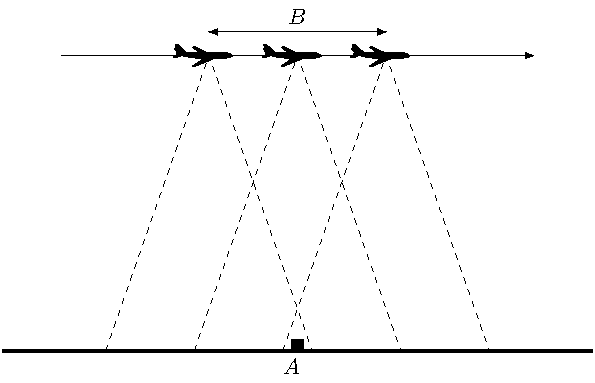
\includegraphics[scale=0.2]{../../Figures/Tesis/Capitulo3/AperturaSintetica.png}}
	%\subfigure{\includegraphics[scale=0.5]{../../Figures/Tesis/Capitulo3/AperturaSintetica2.png}}
	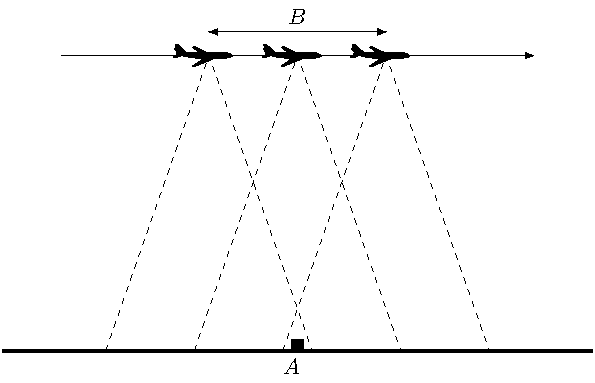
\includegraphics[scale=0.7]{../../Figures/Tesis/Capitulo3/AperturaSintetica.pdf}
	\caption{\label{Apertura}Apertura Sintética en un SAR.} %Fuente Canada Centre for Remote Sensing~\cite{ccrs2001}.}
\end{figure} 


Esta idea de generar una apertura sintética llevó a mejorar la resolución en azimut. La resolución resultante en azimut se vuelve igual a la mitad de la longitud de la antena, es decir, $\Delta x_{\tiny \text{sar}}= \dfrac{L}{2}$.  Observemos que esta resolución es independiente de la longitud de onda y de la distancia al sensor. Además, si se achica la longitud de la antena mejora la resolución.

%La resolución azimutal mejora  considerablemente al considerarse el efecto Doppler que tiene lugar como  consecuencia  del  desplazamiento  del  satélite.  Dos  blancos  puntuales  separados  ligeramente  en  la  dirección azimutal muestran en cualquier instante velocidades relativas algo diferentes (respecto del radar), por  ello,  el  eco  procedente  de  cada  blanco  presentará  un  desplazamiento  en  frecuencia  Doppler  distinto  (Martínez-Benjamin, 1999). El dispositivo SAR puede ser instalado a bordo de un avión o de un satélite.
\subsection{Ecuación del radar}

La ecuación del radar representa la relación que exite entre la energía transmitida y la energía recibida por la antena del radar. Esta relación se define como
\begin{align}
P_r=\dfrac{P_e G^2 \lambda^2 \sigma}{(4 \pi)^3 R^4} 
\end{align}
donde
\begin{itemize}
	\item $P_r$=potencia recibida.
	\item $P_e$=potencia emitida.
	\item $G$=ganancia de la antena (constante adimensional que indica la relación que existe entre la potencia radiada en una dirección y a una distancia, y la  potencia que radiaría una antena isotrópica con la misma potencia emitida y a la misma distancia. Una antena isotrópica es una antena ideal que emite la misma intensidad de radiación en todas las direcciones del espacio.
	$\lambda$=longitud de onda de la señal.
	\item $R$=distancia entre el sensor y el terreno.
	\item $\sigma$= coeficiente de retrodispersión.
\end{itemize}

Entre los parámetros que intervienen en la ecuación del radar se encuentra el coeficiente de retrodispersión $\sigma$. Este parámetro es de interés porque su valor depende de la textura del terreno el cual influye en la intensidad de la señal del retorno.

\section{Formación del ruido Speckle}
\label{FormacionSpeckle}

El láser HeNe es un tipo de fuente que utiliza como medio activo una mezcla gaseosa de helio y neón. De acuerdo a~\cite{Goodman1975,Quel1994} Ali Javan, un físico que trabajaba para Laboratorios Bell Telephone, fue el responsable del funcionamiento del primer láser HeNe en $1960$. Este láser  mostró un fenómeno inesperado: los objetos vistos en luz altamente coherente adquieren una apariencia granular peculiar que no tiene una relación obvia con las propiedades macroscópicas del objeto iluminado, sino que presentan un patrón irregular. 

Esta apariencia granular se conoce como \textit{ruido speckle}. Las imágenes adquiridas por sistemas de iluminación coherente como son las imágenes SAR, las que utilizan laser o ultrasonido entre otros, se ven afectadas por la presencia del ruido speckle. Este tipo de ruido es inherente al proceso de captura de la imagen, no es aditivo ni gaussiano y suele dificultar el análisis e interpretación de las imágenes porque pueden degradarlas significativamente.


%En la teledetección por microondas, la longitud de onda es
%alrededor de centímetros (banda X o C) o decenas de centímetros (banda S, L y P) mientras
%la celda de resolución es de unos metros. Por esta razón, en la misma celda de resolución
%varios dispersores elementales contribuyen al campo total retrodispersado. Todas las ondas electromagnéticas que provienen de la misma celda de resolución se suman de manera coherente y dan como resultado fuertes fluctuaciones en la retrodispersión
%de una celda de resolución a otra~\cite{oliverquegan98}.

En la teledetección por microondas la celda de resolución es de unos metros mientras que la longitud de onda es alrededor de centímetros (banda X o C) o decenas de centímetros (banda S, L y P). Dentro de una celda de resolución existen elementos que dispersan la señal que incide en la celda.

\begin{figure}[hbt]
	\centering    
	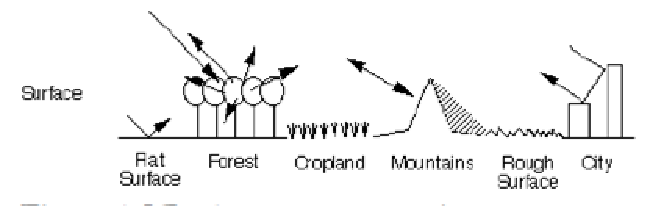
\includegraphics[scale=0.7]{../../Figures/Tesis/Capitulo3/Backscatter.pdf}
	\caption{\label{Backscatter}Radiación reflejada por distintos objetos en la superficie terrestre.}
\end{figure} 

Cuando el radar ilumina una superficie la señal que retorna está compuesta por la suma de los pulsos reflejados por cada uno de los dispersores elementales que se encuentran dentro de la celda, esto se muestra en la figura~\ref{Backscatter}. El tipo de terreno dependerá de la forma en que esta señal se refleje.

Estos dispersores elementales se distribuyen en forma aleatoria y, por lo tanto, la distancia entre ellos y al radar también es aleatoria~\cite{Lee2009}. 
En el momento de la reflexión, la señal que retorna ya no es coherentes en fase pero si lo es en frecuencia. Esto se debe principalmente a la textura de la superficie. La figura~\ref{Reflexion} muestra las señales incidentes y reflejadas en una superficie rugosa. La línea sólida negra corresponde a la primera y la línea punteada roja corresponde a la segunda. La distancia $d$ da información sobre la rugosidad del objeto, la figura~\ref{masrugosa} representa una superficie más rugosa que~\ref{menosrugosa}. Se puede observar que las ondas recibidas son coherentes en frecuencia, pero no necesariamente en fase. Cuanto mayor es el tamaño de $d$ mayor será la diferencia de fase de las ondas reflejadas por los dispersores.

\begin{figure}[hbt]
	\centering    
	\subfigure[]{\label{menosrugosa}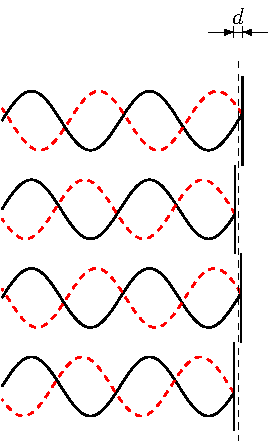
\includegraphics[scale=1]{../../Figures/Tesis/Capitulo3/reflexion_fina.pdf}}\hspace{10mm}
	\subfigure[]{\label{masrugosa}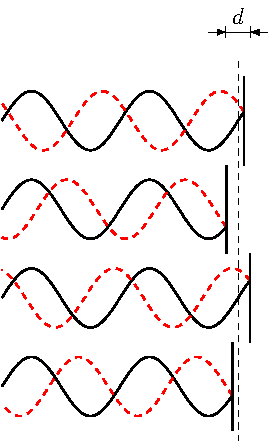
\includegraphics[scale=1]{../../Figures/Tesis/Capitulo3/reflexion_gruesa.pdf}}
	\caption{\label{Reflexion}Coherencia de la señal reflejada.} %Fuente Canada Centre for Remote Sensing~\cite{ccrs2001}.}
\end{figure} 

Entonces, las ondas electromagnéticas que provienen de la misma celda de resolución se suman de manera coherente y dan como resultado fuertes fluctuaciones en la retrodispersión de una celda de resolución a otra~\cite{oliverquegan98}. Por lo tanto el valor de gris en un pixel se obtiene como superposición coherente de las señales incidentes que, al estar desfasadas, pueden interferir de manera constructiva o destructiva, lo que produce que las señales recibidas sean más fuertes o más débiles~\cite{Shahrezaei2019}. Estas interferencias causan variaciones en la magnitud de la señal y cambios aleatorios de intensidad de píxel a píxel. Estos cambios en la intensidad se traducen en la imagen como diferentes niveles de gris. Esto explica el patrón granular que se observa en las imágenes SAR y que produce negros, correspondientes a interferencias destructivas, y puntos brillantes debido a las constructivas~\cite{Yahya2014}. Este patrón angular es lo que se conoce como \textit{Ruido Speckle}.

La presencia de este ruido dificulta la interpretación de las imágenes y puede conducir a interpretaciones y detecciones de bordes erróneas entre otros inconvenientes, debido a la degradación de la calidad de los píxeles. 

Un enfoque común para la presencia de este ruido durante el procesamiento de la señal cruda captada por el radar es promediar varias estimaciones independientes de la señal reflejada. Dado que el radar SAR genera una apertura sintética la longitud de esta antena virtual se puede subdividir en $N$ segmentos independientes, conocidos también como \textit{looks}~\cite{Lee2009}. Cada uno de estos segmentos registra la energía retrodispersada por el mismo blanco y se procesa en forma independientemente para formar una imagen SAR. Estas $N$ imágenes se promedian entre sí para formar una sola imagen SAR de $N$ \textit{looks}. Este procesamiento reduce el efecto del ruido speckle pero, al reducir la longitud de la antena en segmentos, se pierde resolución en azimut. La utilidad de este procedimiento se manifiesta en la mejora de la relación señal-ruido. Cuantas más subdivisiones se hagan, es decir, cuanto más \textit{looks} formen la imagen menos resolución tendrá pero también será menos ruidosa.

\section{Doble Bounce o Doble Rebote}
\label{DobleBounce}
El efecto Doble Rebote es una característica importante que tienen las  imágenes de alta resolución como lo son las imágenes SAR. Este efecto resulta en un fuerte mecanismo de dispersión de la señal emitida por el radar. Aparece por ejemplo, cuando la señal emitida rebota en la calle, luego en los edificios (llamado un doble rebote) como se ve en la figura~\ref{DobleRebote}, o cuando rebota en un edificio y en sus alrededores (corner reflector).  Este efecto se observa en las imágenes SAR como puntos muy brillantes, en cambio, las autopistas aparecen oscuras al ser superficies planas. En la figura~\ref{DobleBounce} se puede ver un esquema de diferentes reflexiones de una señal emitida por el radar.
\begin{figure}[hbt]
	\label{Dispersion}
	\centering    
	\subfigure[ ]{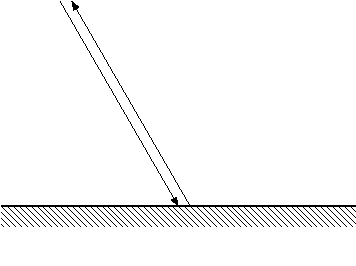
\includegraphics[scale=0.7]{../../Figures/Tesis/Capitulo3/dispersion_a.pdf}}\qquad
	\subfigure[ ]{\label{DobleRebote}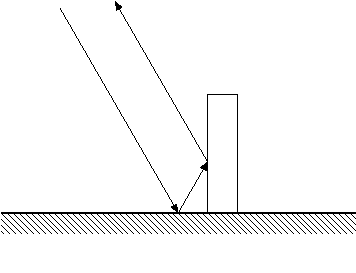
\includegraphics[scale=0.7]{../../Figures/Tesis/Capitulo3/dispersion_b.pdf}}\qquad
	\subfigure[ ]{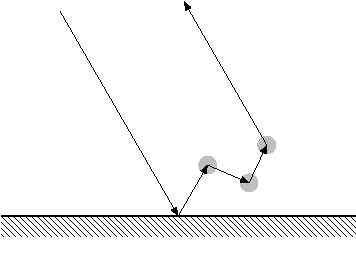
\includegraphics[scale=0.7]{../../Figures/Tesis/Capitulo3/dispersion_c.pdf}}
	\caption{\label{DobleBounce}Diferentes reflexiones de una señal emitida.} %Fuente Canada Centre for Remote Sensing~\cite{ccrs2001}.}
\end{figure} 

Debido a la aleatoriedad y a la fuerte dispersión que puede tener la señal retrodispersada es necesario contar con modelos estadísticos para poder obtener información de las características del suelo.

\section{Retorno Complejo}
\label{RetornoComplejo}

Supongamos que iluminamos un área a través de un haz de energía electromagnética con $n$ dispersores elementales como se mostró en la figura~\ref{SeñalDispersada}. Como presentan Frery y Wu~\cite{FreryLibro2019}, cada dispersor $j$ retornará una fracción de la energía incidente $A_i$ con fase $\phi_i$. El retorno total $S$ es una señal compleja definida por:
\begin{align}
S = \sum_{j=1}^{N} A_j \mathrm{e}^{\mathbf i \phi_j} = 
\underbrace{{\sum_{j=1}^{N} A_j \cos \phi_j}}_{\Re{Z}} +\mathbf i \underbrace{ \sum_{j=1}^{N} A_j \sin \phi_j}_{\Im{Z}}, 
\label{RetornoComplejo}
\end{align}
donde $i$ es la unidad imaginaria y $A_j \mathrm{e}^{\mathbf i \phi_j}$ representa el retorno del $j$-ésimo dispersor. La ecuación~\eqref{RetornoComplejo} describe la suma coherente de las contribuciones del retorno total de cada uno de los dispersores. En general, en vez de tratar directamente con el retorno complejo se trabajan con los datos dados en formato amplitud $A=\mid S \mid$ o  en formato intensidad $I=\mid S \mid^2$, donde $I=A^2$ En esta tesis se trabajará con este último formato.

De acuerdo a~\cite{Quegan1994} si no hay un retrodispersor que domine, la forma de extraer información del retorno de los retrodispersores es aproximándose al problema desde un punto de vista estadístico. Este enfoque se verá en el capítulo~\ref{modeloG0}.



%De esta forma, si consideramos que $N$ es suficientemente grande, podemos apelar al Teorema Central del Límite y pensar que tanto $\Re{S}$ y $\Im{S}$ son variables aleatorias independientes, ambas con distribución $N(0,\sigma^2).$

\section{Conclusiones}

En este capítulo presentamos los conceptos básicos de teledetección, iluminación coeherente y polarización. Estos conceptos son de utilidad porque son el pilar de la formación de imágenes SAR. Se muestran las ventajas y desventajas que poseen estos sistemas frente a aquellos que adquieren imágenes ópticas. Entre las ventajas se encuentran la capacidad que tienen los sensores SAR de adquirir imágenes independientemente de las condiciones climáticas y de la luz, ya que ellos poseen un sistema de iluminación propia. Entre las desventajas se encuentra el ruido speckle que está presente en este tipo de imágenes porque es propio a la forma de adquirir las mismas. 

Asimismo se muestra que el aprovechamiento del efecto Doppler contribuye a generar la apertura sintética del radar SAR. Las bondades de esta apertura sintética se pone de manifiesto en la obtención de imágenes con  mejor resolución.

Finalmente se presenta la aleatoriedad de la formación del ruido speckle, lo que pone de manifiesto la necesidad de encontrar modelos estadísticos que permitan analizar e interpretar este tipo de imágenes.

%En consecuencia, el
%la intensidad y la fase en la imagen final ya no son
%determinista, pero sigue en cambio un exponencial y uniforme
%distribución, respectivamente [5]. La reflectividad compleja total
%para cada celda de resolución viene dada por
%
%El ruido speckle tiene un carácter multiplicativo, es decir, su varianza aumenta con su intensidad~\cite{Moreira2013}. Para reducir la presencia de este ruido se utiliza una una técnica conocida como \textit{multilook}
%ya que se utiliza la apariencia múltiple, que es básicamente una no coherente
%promedio de la imagen de intensidad [2], [5]. Aunque multilook
%provoca una degradación en la resolución de la imagen, en gran medida
%mejora la interpretabilidad de la imagen SAR como puede ser
%visto en las Figuras 5 (b) –5 (d). También el efecto de moteado tiende a
%debilitarse para sistemas de muy alta resolución, ya que el número
%de dispersores elementales dentro de una celda de resolución disminuye.

%\section{Modelo Estadístico}
%
%Los sistemas de iluminación coherente como son los imágenes SAR, el laser y ultrasonido-B entre otras, están afectadas por la presencia del ruido speckle. 
%Con el objetivo de disminuir los efectos de este ruido, se han utilizado filtros como así también una técnica llamada procesamiento multilook.  Esta técnica se aplica a menudo durante el proceso de formación de la imagen y consiste en generar, de forma estadísticamente independientes, varias ``vistas'' o looks a partir del mismo conjunto de pulsos crudos durante el proceso de generación de la imagen. La imagen resultante es la obtenida promediando estas vistas. Tanto el procesamiento multilook como los filtros reducen la presencia del ruido speckle pero se pierde resolución. De esta manera hay un compromiso entre la calidad visual y la presencia de ruido. 
%
%Se han utilizado modelos estadísticos para la comprensión y análisis de imágenes SAR que tienen en cuenta la presencia de este ruido. El modelo multiplicativo considera la presencia del ruido speckle, ya que plantea que el valor observado en cada celda de la imagen es una variable aleatoria $Z$ que resulta del producto de dos variables aleatorias independientes: una correspondiente al backscatter o retrodispersión $X$ y la otra correspondiente al ruido speckle $Y$. Este modelo es el que se propone para modelar datos que provienen de un sistema de iluminación coherente, como son los datos SAR. Este modelo fue propuesto por Frery et al. \cite{Frery97} y permite describir las áreas muy texturadas o texturadas rugosas mejor que la distribución $\mathcal{K}$ \cite{Jakeman87}.

%El modelo multiplicativo considerado es el siguiente:
%\begin{equation*}
%	Z=X \cdot Y  
%\end{equation*}
%donde $X$ e $Y$ corresponden al backscatter y al ruido speckle, respectivamente. La variable aleatoria $Y$ se modela con la distribución $\Gamma ( L,L) $, donde $L\geq 1$ es el número equivalente  de looks, mientras que $X$ sigue una distribución Gaussiana Inversa Generalizada, denotada por  $\mathcal{N}^{-1}( \alpha ,\lambda ,\gamma ) $. De esta forma tenemos que $Z$ obedece una distribución $\mathcal G_I$ \cite{Frery97}.
%Para valores particulares de los parámetros de la distribución $\mathcal{N}^{-1}$ se obtienen las distribuciones $\Gamma ( \alpha ,\lambda ) $,  $\Gamma ^{-1}( \alpha ,\gamma ) $, que llevan a las distribuciones $\mathcal{K}$, $\mathcal{G}_I^{0}$, respectivamente. En esta tesis trabajaremos con la distribución para datos de intensidad denotada por $\mathcal{G}_I^{0}$.
%% % % ¿Tiene sentido darle una notación a una distribución sin saber de qué parametrización se trata?
%
%Su función de densidad está dada por
%\begin{equation*}
%	f_{\mathcal{G}_I^{0}}( z) =\frac{L^{L}\Gamma ( L-\alpha
%		) }{\gamma ^{\alpha }\Gamma ( -\alpha ) \Gamma (
%		L) }\cdot  
%	\frac{z^{L-1}}{( \gamma +zL) ^{L-\alpha }},%
%	\label{ec_dens_gI0}
%\end{equation*}
%donde $-\alpha,\gamma ,z>0$ y $L\geq 1$.

%Bajo este modelo se pueden caracterizar regiones con diferente grado de textura a través de los parámetros de la distribución $\mathcal{G}_I^{0}$. Para valores de $\alpha$ cercanos a cero (típicamente en el intervalo $(-3,0)$), la zona de la imagen corresponde a una región muy texturada, como es el caso de las zonas urbanas en las imágenes SAR. A medida que el valor del parámetro $\alpha$ disminuye, corresponde a zonas con cada vez menos textura, como son las regiones de forestación (usualmente $(-6,-3]$) y pastura (en $(-\infty,-6)$). Por otro lado, el parámetro $\gamma$ (llamado parámetro de escala) posee una interpretación en términos del brillo. Cuanto mayor es su valor, mayor intensidad posee la imagen en esa región. Por estas razones, la estimación precisa de los parámetros, en particular el parámetro de textura, es de suma importancia en el análisis de imágenes con ruido speckle. 
%
%%\section{Antecedentes}
%En los últimos años se han propuesto varios métodos de estimación de parámetros, Vasconcellos et al.~\cite{VasconcellosFrerySilva:CompStat} cuantifican el error en la estimación del parámetro de textura para la distribución $\mathcal G_A^0$ y proponen una técnica analítica para mejorar la estimación.
%Silva et al.~\cite{SilvaCribariFrery:ImprovedLikelihood:Environmetrics} proponen otro método analítico para mejorar la estimación del parámetro de textura que reduce el error cuadrático medio.
%Cribari-Neto et al.~\cite{CribariFrerySilva:CSDA} proponen el uso de bootstrap para el mismo fin. 
%Allende et al.~\cite{AllendeFreryetal:JSCS:05} y Bustos et al.~\cite{BustosFreryLucini:Mestimators:2001} plantean mejoras para la estimación del parámetro de textura, pero con foco en su robustez. 
%
%%Entre las técnicas de estimación paramétrica clásicas se encuentran las de máxima verosimilitud y momentos. Recientemente en ~\cite{MellinAnalysisPolSAR,BujorTrouveValetNicolas2004,khan2014} han propuesto estimadores del parámetro de textura basado logcumulants y logmomentos, donde interviene la transforamda de Mellin de la función de densidad. En Tison et al.~\cite{Tison2004} los autores mostraron que los estimadors de los parámetros de la distribución $\mathcal G^0$, para datos de amplitud, mejoran al estimador de máxima verosimilitud.
%%
%%Es importante mencionar que, entre las propiedades que se espera que un buen estimador posea, son la consistencia, insesgadez, eficiencia, robustez y normalidad asintótica. Son conocidas las buenas propiedades asintóticas que posee el estimador de máxima verosimilitud. 
%%Sin embargo, en algunas situaciones como es el caso de la estimación del parámetro de textura de la distribución $\mathcal G_I^0$, este estimador no se comporta adecuadamente para el caso donde el tamaño de muestra es chico. 
%%% % % ACF Puede no ser verdad siempre.
%%Es importante considerar este caso ya que muchos de los métodos de filtrado de imágenes o detección de bordes utilizan máscaras deslizantes de tamaño $3 \times 3$,  $5 \times 5$, $7 \times 7$, $9 \times 9$ or  $11 \times 11$. Por eso es de interés encontrar buenos estimadores de los parámetros de la distribución $\mathcal{G}_I^0$ para el caso de muestras de pequeño tamaño. 
%
%Por otro lado, la teoría de la información ha sido aplicada a los métodos de estadística y probabilidades con éxito~\cite{Liese2006}. 
%Shannon~\cite{Shannon1948} definió la información $I(X,Y)$ entre las variables aleatorias $X$ e $Y$ como una divergencia calculada entre sus densidades de probabilidad. 
%Estas divergencias fueron ampliamente estudiadas por Kullback y Leibler~\cite{KullbackLeibler1951} y por Rényi~\cite{renyi1961} entre otros y es una medida de la distancia entre dos funciones de densidad. 
%%El concepto de divergencias como distancias estocásticas se describe detalladamente en~\cite{Liese2006}, así como también sus propiedades.  
%% Mejorar las referencia en eventos con artigos en periódicos
%Este tipo de divergencias poseen múltiples aplicaciones en procesamiento de señales e imágenes~\cite{4218961}, análisis de imágenes médicas~\cite{5599869},
%clasificación de texturas~\cite{1246862}, restauración de imágenes~\cite{1224731} e incluso en detección automática de regiones con diferente grado de rugosidad en imágenes SAR~\cite{6377288,ClassificationPolSARSegmentsMinimizationWishartDistances}.
%
%% % % ACF Hace falta conectar mejor el párrafo anterior con este
%%\textcolor{red}{\sout{Los estimadores del kernel clásico~\mbox{\cite{Silverman1986}} son populares en la estimación de la función de densidad. Sin embargo, si la densidad a estimar tiene soporte acotado, estos estimadores pueden dar estimaciones sesgadas en los bordes del soporte porque asignan probabilidad positiva fuera del soporte de la función. 
%%Una alternativa para mejorar esto es utilizar kernels asimétricos, Chen~\mbox{\cite{chen1999, chensx2000}} presenta núcleos Beta y Gamma, Scaillet~\mbox{\cite{Scaillet2004}} introduce núcleos Inverso Gaussianos (IG) y Recíproco Inverso Gaussiano (RIG), Bouezmarni et al.~\cite {bouezmarni2005} demuestran propiedades teóricas de los núcleos Gamma, IG y RIG. En~\cite{Jin2003} los autores proponen los núcleos Birnbaum-Saunders (BS) y Lognormal (LN). Es interesante señalar que  estos estimadores varían su forma de acuerdo con la observación, una característica que permite obtener diferentes grados de suavizamiento sin incurrir en los problemas antes mencionados~\cite{Scaillet2004}.}}
%
%
%%\section{Hipótesis de trabajo}
%En esta tesis se propone estudiar un nuevo  estimador de los parámetros de la distribución $\mathcal{G}_I^0$ definido como el punto del espacio paramétrico que minimiza la distancia estocástica que existe entre la función de densidad teórica $\mathcal{G}_I^0$ y una estimación no paramétrica de la función de densidad subyacente. 
%
%Dentro de los estimadores no paramétricos de la función de densidad subyacente se encuentran los estimadores de kernel clásico, con kernel simétrico~\cite{Silverman1986} que son populares en la estimación de la función de densidad.
%Sin embargo, si la densidad a estimar tiene soporte acotado, estos estimadores pueden dar estimaciones sesgadas en los bordes del soporte porque asignan probabilidad positiva fuera del soporte de la función.
%Una alternativa para mejorar esto es utilizar kernels asimétricos, Chen~\cite{chen1999, chensx2000} presenta núcleos Beta y Gamma, Scaillet~\cite {Scaillet2004} introduce núcleos Inverso Gaussianos (IG) y Recíproco Inverso Gaussiano (RIG), Bouezmarni et al.~\cite {bouezmarni2005} demuestran propiedades teóricas de los núcleos Gamma, IG y RIG. En~\cite{Jin2003} los autores proponen los núcleos Birnbaum-Saunders (BS) y Lognormal (LN). Es interesante señalar que  estos estimadores varían su forma de acuerdo con la observación, una característica que permite obtener diferentes grados de suavizamiento sin incurrir en los problemas antes mencionados~\cite{Scaillet2004}. En esta tesis se propone estimar la función de densidad subyacente utilizando núcleos asimétricos.
%
%% % % Esperanza unitaria es algo muy técnico que no debería estar en la propuesta.
%
%%\textcolor{red}{\sout{Se propone entonces estimar el parámetro $\alpha$, denotado $\widehat\alpha_{\text{\tiny{K}}}$ considerando $Z_1, \ldots, Z_n$ un conjunto de $n$ variables aleatorias independientes e idénticamente distribuidas que siguen el modelo $\mathcal{G}_I^{0}(\alpha,\gamma^*,L) $, donde $\gamma^* $ se elige de modo que $E(Z)= 1$.
%%Sea $\widehat{f}_{K}$ una estimación no paramétrica, con núcleo asimétrico $K$, de la función de densidad subyacente. El estimador $\widehat{\alpha}$ está dado por la minimización de la siguiente ecuación:}}
%%\begin{align}
%%\textcolor{red}{\sout{\widehat{\alpha}_{K}= \arg\min_{\alpha} d\big(f_{\mathcal{G}^{0}}(\alpha,\gamma^*, L ), \widehat f_K(z)\big),}}
%%\label{minimization}
%%\end{align}
%
%Se comparará el desempeño de este estimador, en términos de sesgo y error cuadrático medio y tasa de convergencia, con los presentes en la literatura. Se estudiarán las propiedades de este estimador, como así también la robustez del mismo bajo diferentes esquemas de contaminación.
%
%%Entre las alternativas no paramétricas de estimación de la función de densidad se encuentra el estimador kernel (núcleo) utilizando núcleos simétricos. Este estimador es ampliamente utilizado y posee buenas propiedades, pero cuando la función de densidad tiene soporte acotado, como es el caso de la $\mathcal{G}_I^0$, utilizar este tipo de núcleos puede conducir a estimaciones sesgadas ya que ellos asignan probabilidad positiva a valores que se encuentran fuera del soporte de la distribución.
%%
%%Algunos autores proponen utilizar núcleos asimétricos para resolver este problema. Chen~\cite{chen1999,chensx2000} presenta los núcleos Beta y Gamma,~\cite{Scaillet2004} introducen los núcleos Inverso Gaussiano y Recíproco Inverso Gaussiano. En~\cite{bouezmarni2005} los autores muestran que estos estimadores poseen buenas propiedades. 
%%
%%Esta tesis propone estimar la función de densidad subyacente utilizando núcleos asimétricos como paso previo a la obtención de los estimadores de los parámetros de la distribución a través de la minimización de la distancia estocástica. 

% \section{Backscatter}
%
%Sacado de SARMAP
%Retrodispersión para un área objetivo a una longitud de onda particular variará para una variedad de condiciones,
%tales como el tamaño físico de los dispersores en el área objetivo, las propiedades eléctricas del objetivo
%y el contenido de humedad, con objetos brillantes que aparece más húmedas y secas objetivos que aparecen
%oscuro. (La excepción a esto es un cuerpo suave de agua, que actuará como una superficie plana y
%reflejar pulsos entrantes y lejos del sensor. Estos cuerpos aparecerán oscuros). la longitud de onda
%y la polarización de los pulsos de SAR, y el ángulo de observación también afectarán retrodispersión.
